%!TEX root = ../main.tex

This section covers the steps needed to produce the wanted results. The input needed is a fiducial marker $M$ to provide the object position in the real world; and a 3D mesh $O$ which will be rendered in Augmented Reality. The output is a set of light sources $L_i$, each one having a position, orientation, intensity, color, type and size. In order to complete the luminance ($L()$) analysis a 360 panoramic image is required, but it will be generated as a previous step, it is not necessary to have one beforehand. The entirety of the process is layed out in the flowchart in Figure 1, and each step is described in more detail afterwards.

\begin{figure}[H]
  \centering
  \setlength{\unitlength}{\textwidth} 
    \begin{picture}(1,0.5)
       \put(-0.1,0){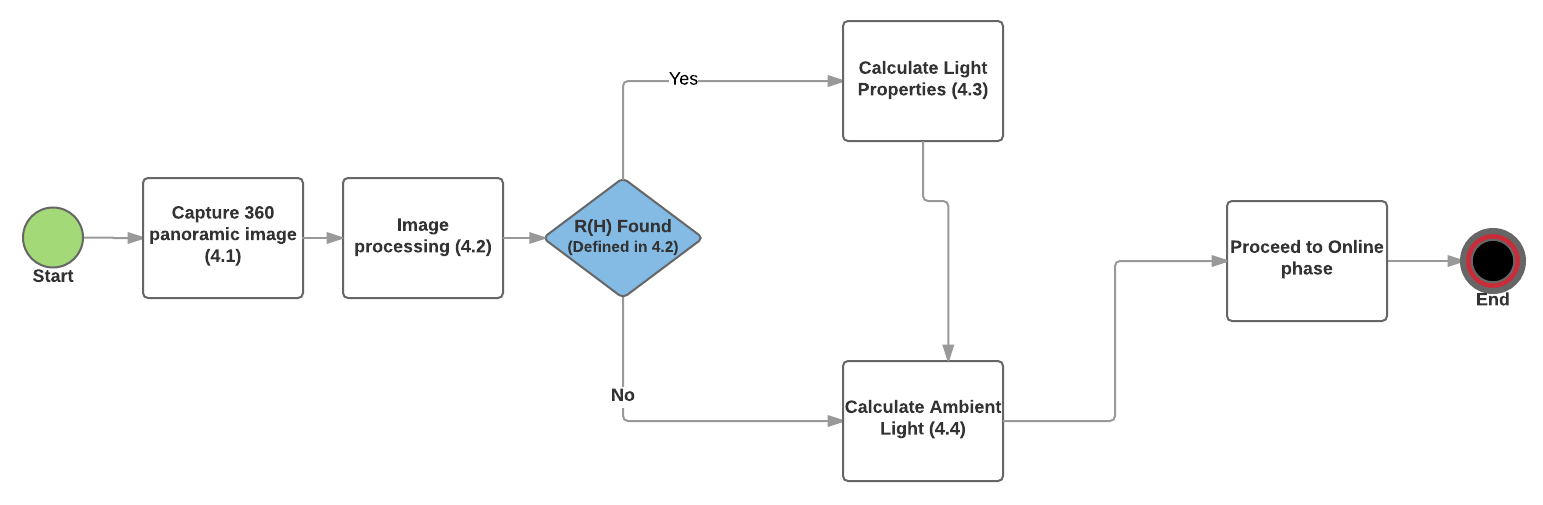
\includegraphics[width=1.3\unitlength]{Figures/Flowchart.png}}
       
    \end{picture}
    \caption{The method in a nutshell}
\end{figure}

\section{Capture 360 panoramic image}
In this work panoramic images are used as a tool, therefore it's not within the scope of the method to define a new way of capturing 360 images. The implementation will be based on the one by Chuang et al. \cite{ThreeSixty}
$M$ will provide the origin of the virtual world for placing and orienting $O$ within it. In order for the lights to be mapped to the same position as $M$ the user will be asked to place the marker in the desired position and start capturing the environment while the marker is centered in frame. This will also simplify calculations of light orientations later on.

\section{Image processing}
Once the panoramic image exist the first step in order to be able to analyze the luminance is to get rid of the chromatic information. This is achieved with the following equation:

\begin{equation}
    L(R_{ij},G_{ij},B_{ij}) = 0,2126 \times R_{ij} + 0,7152 \times G_{ij} + 0,0722 \times B_{ij}; \quad \forall \  P_{ij}
\end{equation}

Where $L$ is the luminance obtained at D65 white point and $P$ is the pixel in the $i,j$ position of the image \newline
The contrast ratio has to be adjusted, so that the regions with high luminance are more clearly differentiable. 

\begin{equation}
     g(i,j) = \alpha \times f(i,j) + \beta
\end{equation}

Where $g(i,j)$ is the adjusted image, $f(i,j)$ is the original grayscale image and $\alpha$ and $\beta$ are the brightness and contrast constants, determined by parameter tuning. The parameter tuning will be carried out in a trial and error way, propose initial extreme values and run the program, changing the values in order to achieve the best result.
In order to prevent outlier pixels and noise from causing false positives, let $g(i,j)$ be normalized like so:

\begin{equation}
    L(P_{ij}) = \frac{ 2 \times P_{ij} }{min(L) + max(L)}
\end{equation}

Where $min(L)$ and $max(L)$ are the overall minimum and maximum luminance values in the image. 
\newline
The result of these steps is a black and white image with the rough shape of the light source. If the image ends up completely black it means there are no important visible light sources and ambient illumination alone would give a good enough result on the rendered model. A region of high luminance is defined as follows:

\begin{equation}
    R(H) = \{p_{00}, p_{01}, ... , p_{mn}\}
\end{equation}
 Where $p_{ij}$ is the pixel in the i,j position of the image. Such that 
\[
    L(p_{ij}) > 0.9 \times max(L(p_{ij})) 
\]

The region must also be continuous, so the pixels must be adjacent.\newline
If there are regions of high luminance in the image, they would be discovered with a fair amount of noise and artifacts, caused by clear objects, reflections of light sources on highly reflective surfaces, or even light sources that are so far away in the distance that don't really contribute an important amount of light to the area of interest. Therefore it's necessary to also add a relative size constraint to the definition. What constitutes an acceptable region size to deem the light source is not an easy question to answer. The best approach to face this problem is to define it as a percentage of the width and height of the overall image and tune the parameter in search for the best solution. The size constraint would therefore be:

\begin{equation}
    width(R(H)) \times height(R(H)) \geq k \times W \times H
\end{equation}

Where $k$ is the parameter to be tuned; $W$ and $H$ are the total image width and height.\newline

These constraints also help keep the amount of lights to be processed within an acceptable range for a real-time application, even if the real environment has many light sources a simplification of them is necessary when modelling them to keep the application feasible. Once the relevant light sources have been identified their properties need to be calculated.

\section{Calculate light properties}
The properties needed to calculate for each light are position, orientation, intensity, size and color. In the real world it is not trivial to calculate the position and size at the same time, because at least one of them would have to be known. Fortunately in the virtual world this is not necessary, as long as it is consistent, for the area size of the light the pixel measures can be used. With this in mind all the other properties can be calculated.

\begin{enumerate}
\item Width and height: The pixel measures will be used for this, they can me determined from the size constraint in the previous step.
\item Position: It is posible to calculate the distance from and object to a camera lens knowing a few parameters from the lens, namely the focal lenght and the sensor size. In Android these values are easily obtainable through the ExifInterface class. In iOS the values are publicly known per device family, so it's possible to create a lookup table with the values and have the application ask what device it's running on to match the necessary set of values. The calculation is then done as follows:

\begin{equation}
    d(L_i) = \frac{ f \times h_i}{sensorHeight}
\end{equation}

\item  Orientation: Since the user was enforced to capture the environment starting from the north and the environment is the entire 360 degrees it is easy to map the pixel width to the angle of incidence of the light source. We can for example define the following ratio to calculate the angle:

\begin{equation}
    \phi = \frac{pos(L_i)_x \times 180}{imageWidth \times 0.5}
\end{equation}

\item Color: Storing both versions of the panorama, one in full color and another one after processing will allow us to have both the color and the luminance information. Once a light source is detected, the equivalente area in the color image can be averaged to determine the color of the light source.
\item Type: There are two main shapes of lamps in the real world, quadrilateral and elliptical. It is indeed possible to find lights with more complex shapes, however, as long as the area of emission is the same, simplifying it to a quadrilateral or elliptical shape yields the same result for the purposes of the method.
\newline 
Determining if the light is a spotlight or an area light will be done through the shape. Elliptical lights will be tagged spotlights and quadrilateral lights area light. Shape detection will be carried out using OpenCV contour detection and counting the vertices of the contour. Even if in the real world the light is a perfect square and the camera is facing it with no parallax it is expected that,  due to artifacts and noise, the function may not find exactly 4 vertices. This is not a big problem, because the number of vertices needed to create smooth circle range in the dozens. So adjusting a threshold value is a simple and acceptable solution.
\end{enumerate}

\section{Calculate ambient light}
Environment mapping is an image-based technique to approximate the appearance of the overall light conditions of an environment. This is accomplished by means of a precomputed texture image mapped as a far-away environment surrounding. Said surrounding is usually a geometric surface, when Blinn first introduced the method\cite{Blinn76} a sphere was used. Nowadays there are other alternatives, such as cube, paraboloid, pyramid or cylinder maps. The principle for each surface is the same, but the way to map a planar image onto the surface varies per surface.\newline
Since a panoramic image of the environment is already available using it to implement environment mapping would be an adequate use of resources. In order to generate an environment map it is necessary that the panorama is made into a High Dyamic Range image. This is because the Low Dynamic Range image captured directly from the device camera fails to capture the information necessary to simulate correct color balance, shadows, and highlights of the lighting environment; ultimately producing both inaccurate and less visually pleasing results. This has been illustrated by Paul Debevec.\cite{DebevecRSO}\newline 
A relatively easy and effective way to make an image into an HDR version is a technique called Tone Mapping, in which versions with different exposure values of the same image are blended together to include the full range of highlights and shadows of the overexposed and underexposed versions in a single image. Since asking the user to capture the environment more than once would have a bad impact on user friendliness, and also it's highly unlikely that the produced image would have the exact same framing every time, the different exposure values for the Tone Mapping will be produced altering the brightness and contrast values of the base image using equation 2 once again. After that the HDR image is produced using Debevec's weighting algorithm\cite{Debevec}.\newline
It's important to disclaim that the Tone Mapping process will not yield an actual HDR image. In the first place, it will be a standard 24 bit image in the $0...255$ range, with highlight and shodow valued clipped. The upside to still going through this process nonetheless is that the environment will be described in a richer way, capturing the bright areas and the shodows better than the standard exposure image.\newline
After the HDR version of the panorama is created it can be used to have an actual ground truth about the environment light color and intensity at any given point in the virtual space. This will be detailed in the Real-time Phase step subsection.

\section{Real-time Phase}
Everything proposed in the method may be accurate and could theoretically yield more convincing AR rendering, but it has to be tested in order to determine for sure if that is the case. That is the motivation for implementing a tailor made AR application where all actors come into play to prove or disprove the accuracy and feasibility of the composited virtual objects in the camera feed.\newline
The system is intended to work with ARToolkit, which already has implemented an OpenGL ES 2.0 and an OpenSceneGraph context. OpenGL ES 2.0 allows for great flexibility for lighting, due to the fact that it doesn't have a fixed functionality way to make lighting, a custom made shader has to be made. All the fixed functionality variables from OpenGL, such as the gl\_LightSource array are gone, left for every developer to implement the shader inputs and outputs however they see fit. So there won't be any concerns about getting the light parameters that OpenGL understands, the shader will just read an array of data and as long as the logic is well implemented everything will just work.\newline
The virtual side of the application will have the set of lights, the model $O$ to display and the HDR environment mapped into a cylinder. For the object, a matte diffuse shader, a shiny plastic-like shader and a reflective metal-like shader will be implemented. For performance concerns a refractive glass-like shader or Fresnel effect will not be present. The cylinder with the environment will not be rendered as such, but it will be used to calculate the environment lighting and reflections on the shaders that have reflectivity, to emulate the effect of a raytracer within the OpenGL rasterizer. This effect is achieved with a per-vertex lighting shader.  The reflected color is calculated with the normal vector at a vertex of the surface, and the view vector. The reflection is calculated like so:
\begin{equation}
    R = I - 2\times dot(N,I) \times N
\end{equation}
Where $I$ is the view vector and $N$ is the current vertex normal. GLSL has a shorthand method for equation 8 called reflect().
The light ray that is reflected by the object at the current point of the surface is same as R vector, so using it the color from the environment can be obtained and finally the reflected color is mixed with diffuse color of the object in the proportion defined in the material parameters. \newline
After the color of $O$ the influence of the light sources calculated on the pre-calculation phase on the current vertex will be calculated using Lambert's cosine law.